\section{Burst signals, SNR and injections}\label{sec:signals}

\subsection{Morphologies}
Three phenomenological morphologies are injected (Table~\ref{tab:morph}); all have closed-form Fourier transforms (Gaussian integrals with complex width), which are implemented exactly and checked against a brute-force numerical transform
(agreement to $10^{-4}$ or better for all three).
\begin{table}[h]\centering\small
\begin{tabular}{llp{4.6cm}}
\toprule
morphology & $h(t)$ & injection prior\\
\midrule
sine-Gaussian (SG) & $e^{-t^2/2\sigma^2}\cos(2\pi f_0t+\phi)$, $\sigma=Q/2\pi f_0$ & $f_0\sim$ log-U(50,400)\,Hz, $Q\sim$ U(4,15)\\
Gaussian pulse & $e^{-t^2/2\sigma^2}$ & $\sigma\sim$ log-U(0.8,5)\,ms\\
linear chirp & $e^{-t^2/2\sigma^2}\sin(2\pi f_0t+\pi\dot ft^2+\phi)$ & $f_0\sim$ U(50,150)\,Hz, $\dot f\sim$ U(150,600)\,Hz/s, $\sigma\sim$ U(30,80)\,ms\\
\bottomrule
\end{tabular}
\caption{The three burst morphologies. For all of them $t_0\sim$ U(0.25,0.75)\,s inside the one-second window and $\phi\sim$ U(0,$2\pi$).}\label{tab:morph}
\end{table}

\subsection{Injection chain and validation}
Signals are not added in the time domain after whitening. They are built directly as whitened frequency bins $V_k=2\tilde h(f_k)/\sqrt{S_n(f_k)}$ with the PSD of the chunk of the host window and added to the real whitened bins.
This is equivalent to injecting in the strain (whitening is linear), gives the exact optimal SNR of Eq.~\eqref{eq:snr} and has no filter transients. The exploratory notebook used the time-domain proxy
``$L_2$ norm of the whitened waveform over the noise standard deviation''; it agrees with Eq.~\eqref{eq:snr} up to the constant factor $1/0.95$ (the noise standard deviation) for all morphologies, and was replaced by the analytic definition.

The chain is validated on real noise: injecting sine-Gaussians at $\snr=0,5,10$ in $4000$ test windows and matching with the exact template, $|z|^2$ follows a non-central $\chi^2_2(\snr^2)$ law
(means $2.03$, $27.1$, $101.8$ against $2$, $27$, $102$; Kolmogorov--Smirnov $p=0.64,0.66,0.49$). Figure~\ref{fig:inj} shows what the injections look like.

\begin{figure}[h]\centering
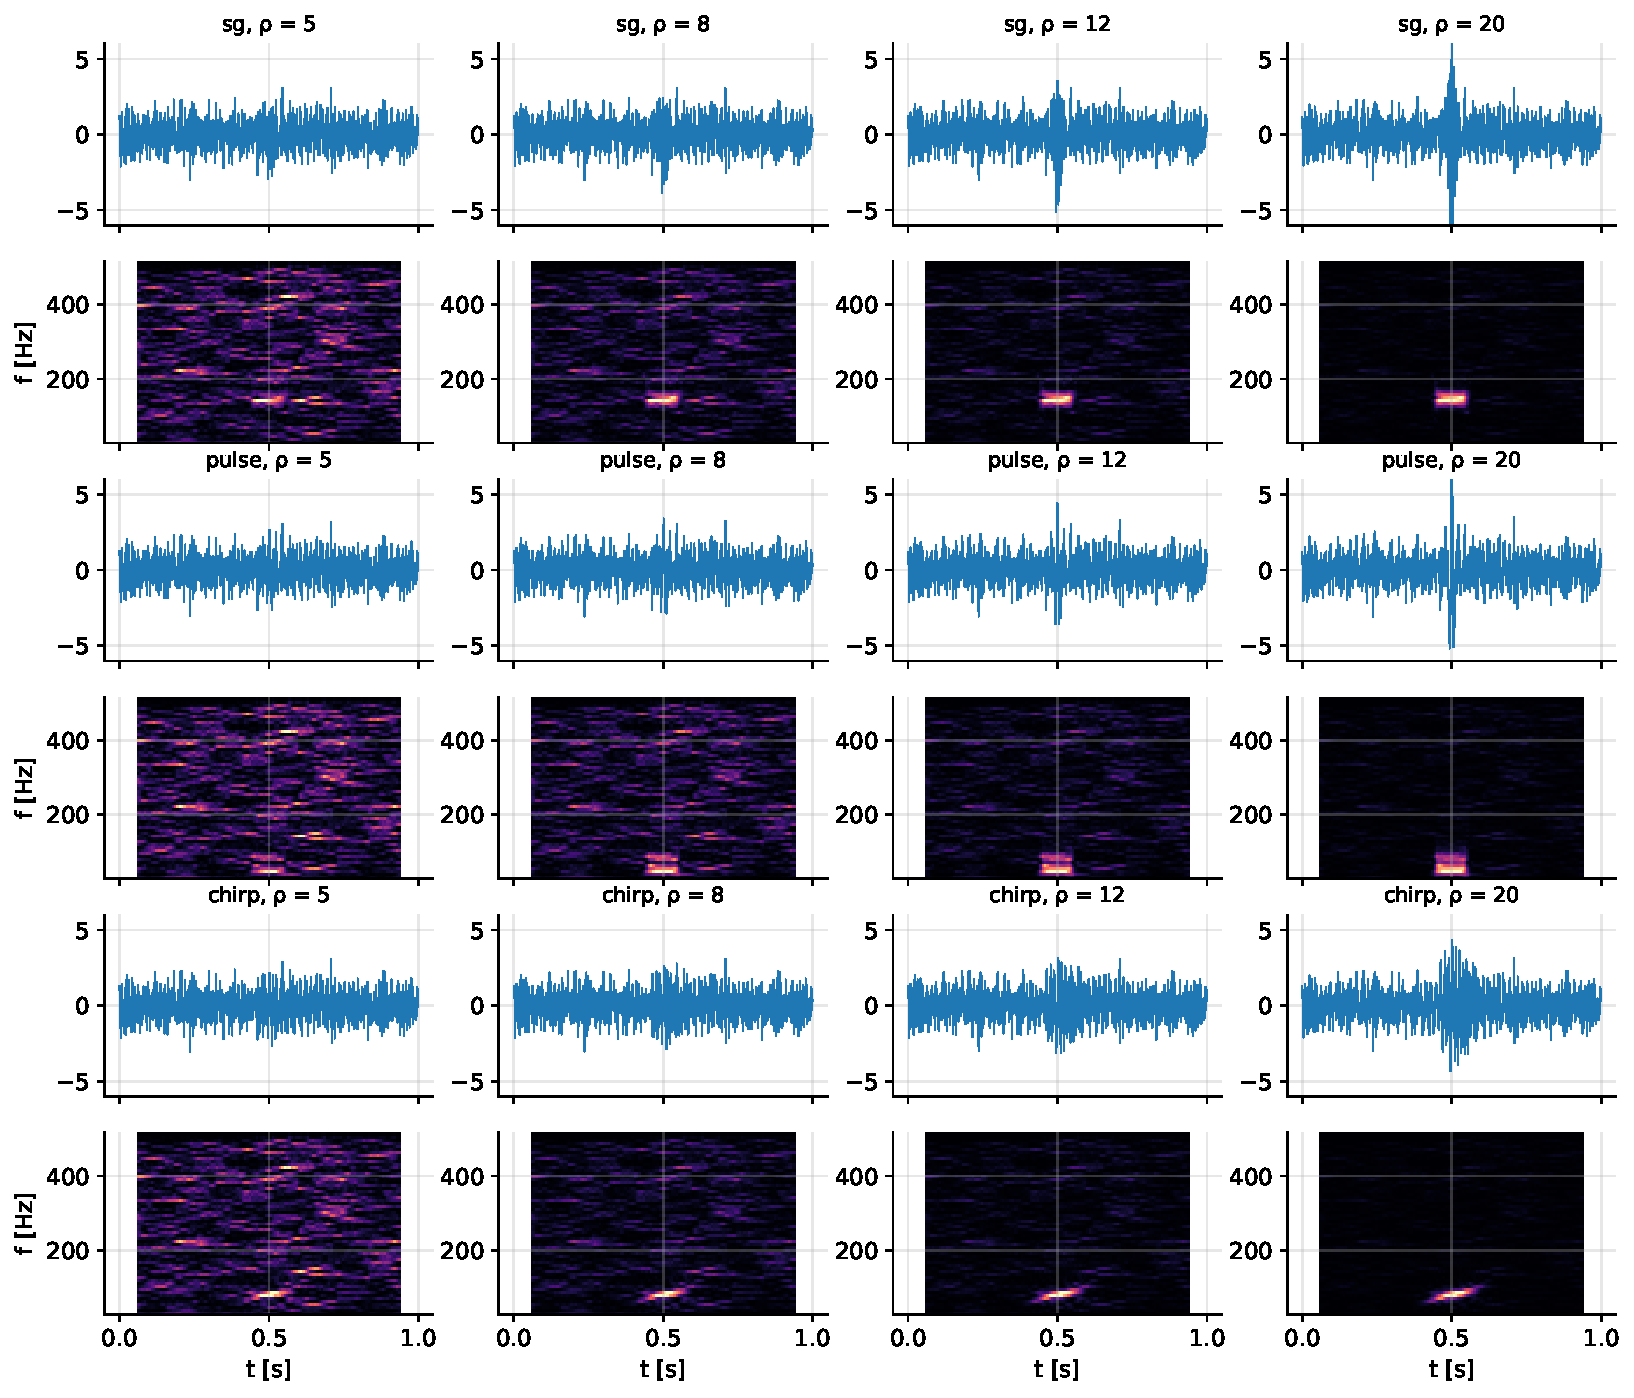
\includegraphics[width=0.78\textwidth]{fig02_injections_tf.pdf}
\caption{The three morphologies injected into the same real noise window at $\snr=5,8,12,20$: whitened series (top row of each pair) and spectrogram (bottom). At $\snr=5$ nothing is visible by eye.}\label{fig:inj}
\end{figure}
